\subsection{Présentation de l'entreprise}
    Forssea Robotics est une jeune entreprise innovante en matière de robotique sous-marine. Elle propose des solutions industrielles à l'exploration de ce milieu particulièrement hostile à l'homme. Ils excellent principalement dans quatre domaines : la robotique autonome, l'ingénierie des \gls{ROV}s, la vision sous-marine et l'intelligence artificielle. Cette expértise leur vaut de travailler aux côtés de nombreux partenaires, comme le groupe Total, Thales, iXblue, DeepOcean, et bien d'autres, mais aussi avec des centre de recherches comme l'\gls{ENSTAB}.

\subsection{Présentation des produits}
    Forssea Robotics propose deux \gls{ROV}s\footnote{\url{https://forssea-robotics.fr/index.php/products/rovs}}, \gls{Argos} et \gls{Atoll}, visibles sur la \textsc{Figure}~\ref{fig:ROVs}. \gls{Argos} est un robot d'intervention léger intelligent permettant d'embarquer une charge utile pesant jusqu'à $30\ kg$, tandis qu'\gls{Atoll} est un robot de levage autonome qui peut porter porter jusqu'à $1500\ kg$. Il permet de déplacer et de positionner des \gls{frameLBL} sur les fonds marins utilisées dans la localisation sous-marine~\cite{milne1983underwater}. Une \gls{frameLBL} portant une balise est aussi visible sur la \textsc{Figure}~\ref{fig:ROVs}.

    \begin{figure}[!htb]
        \centering
        \begin{subfigure}[b]{0.3\textwidth}
            \centering
            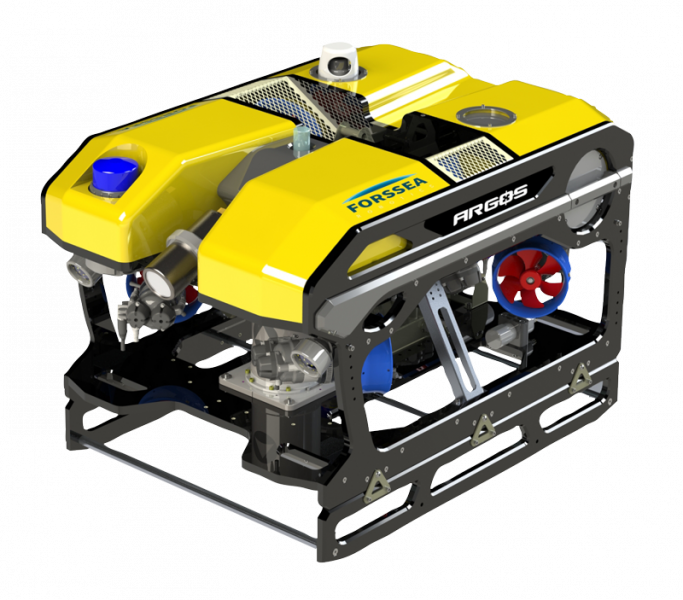
\includegraphics[width=\textwidth]{imgs/Argos.png}
            \caption{\gls{Argos}}
        \end{subfigure}
        \hfill
        \begin{subfigure}[b]{0.3\textwidth}
            \centering
            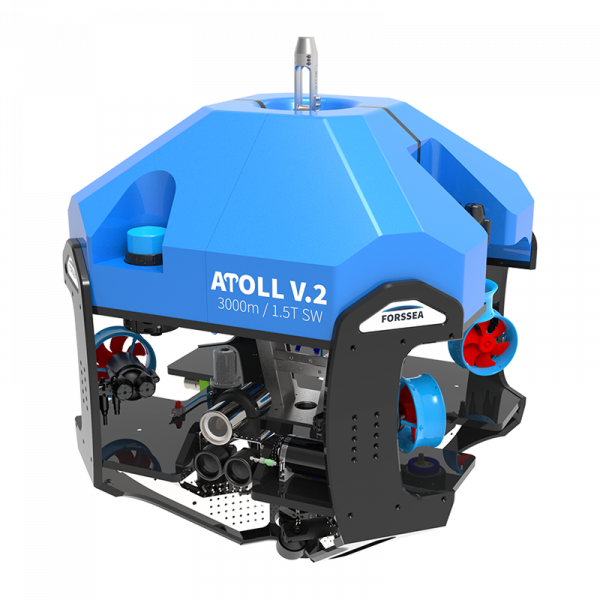
\includegraphics[width=\textwidth]{imgs/Atoll.png}
            \caption{\gls{Atoll}}
        \end{subfigure}
        \hfill
        \begin{subfigure}[b]{0.3\textwidth}
            \centering
            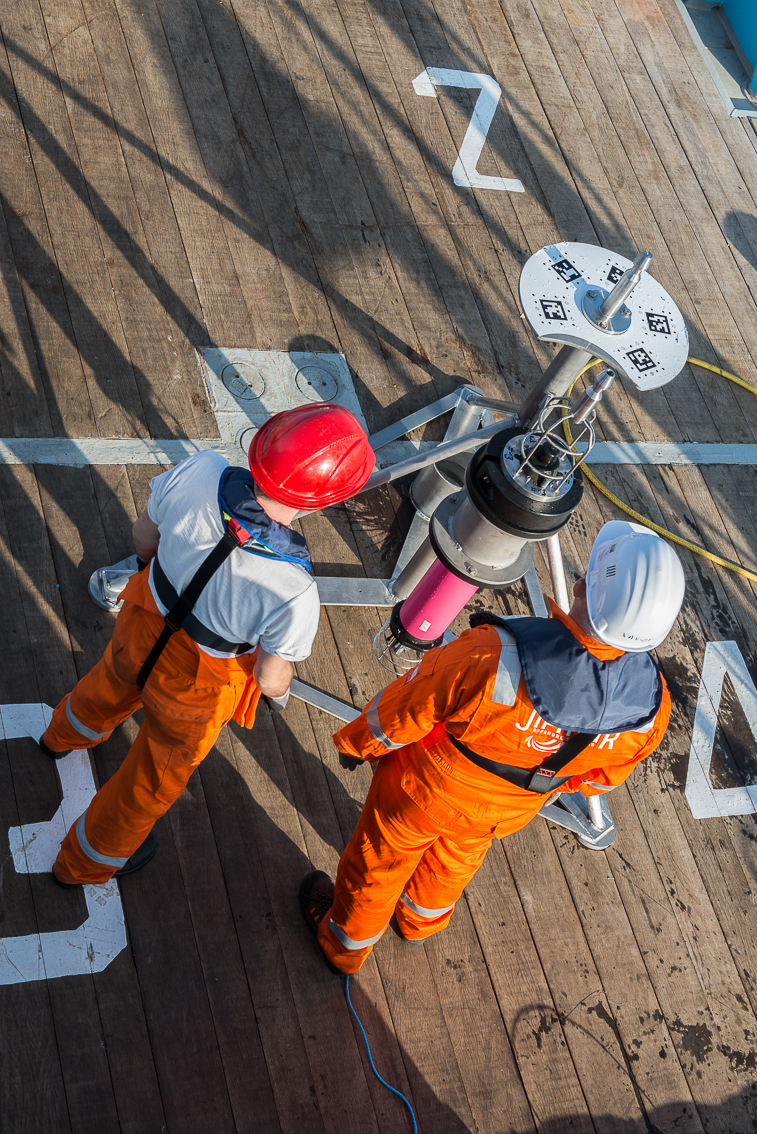
\includegraphics[width=\textwidth]{imgs/Frame.jpg}
            \caption{\gls{frameLBL}}
        \end{subfigure}
        \caption{\gls{ROV}s proposés par Forssea Robotics et \gls{frameLBL}}
        \label{fig:ROVs}
    \end{figure}

    Ils proposent aussi plusieurs solutions de captations visuelles\footnote{\url{https://forssea-robotics.fr/index.php/products/cameras}}. Il y a la \gls{Navcam} qui est une caméra embarquant des algorithmes de traitement permettant de réaliser du positionnement visuel, et l'\gls{Obscam} qui est une simple caméra étanche.